%\listfiles
\documentclass[11pt]{article}
\usepackage{fullpage}
\usepackage{amssymb}
\usepackage{graphics, graphicx}
\usepackage{fancyhdr}
\usepackage{subfigure}
\usepackage{ifthen}
\usepackage{version}
\usepackage{tocbibind}
\usepackage{makeidx}
\usepackage{natbib}
\usepackage{booktabs}
\usepackage[colorlinks=true, pdfstartview=FitV, linkcolor=blue, 
            citecolor=blue, urlcolor=blue]{hyperref}
 
 
 
 \usepackage{bera}% optional: just to have a nice mono-spaced font
\usepackage{listings}
\usepackage{xcolor}

\colorlet{punct}{red!60!black}
\definecolor{background}{HTML}{EEEEEE}
\definecolor{delim}{RGB}{20,105,176}
\colorlet{numb}{magenta!60!black}

\raggedbottom
\sloppy

\parindent=0pt
\parskip=5pt

%\def\MEGANServer{{\sf MEGANServer}}
%\def\MEGAN{{\sf MEGAN}}
\newcommand{\ignoreDB}[1]{}
\newcommand{\prop}[2]{\texttt{\textcolor{blue}{#1}=\textcolor{red}{#2}}}


%%%%%%%%%%%%%%%%%%%%%%%%%%%%%%%%%%%%%%%%%%%%%%%

%%%%%%%%%%%%%%%%%%%%%%%%%%%%%%%%%%%%%%%%%%%%%%%

%%%%%%%%%%%%%%%%%%%%%%%%%%%%%%%%%%%%%%%%%%%%%%%
\title{User Manual for \sf{MEGANServer}1.0}
%%%%%%%%%%%%%%%%%%%%%%%%%%%%%%%%%%%%%%%%%%%%%%%

%%%%%%%%%%%%%%%%%%%%%%%%%%%%%%%%%%%%%%%%%%%%%%%
\author{Hans-Joachim Ruscheweyh}
%%%%%%%%%%%%%%%%%%%%%%%%%%%%%%%%%%%%%%%%%%%%%%%

\makeindex



%%%%%%%%%%%%%%%%%%%%%%%%%%%%%%%%%%%%%%%%%%%%%%%
\begin{document}
%%%%%%%%%%%%%%%%%%%%%%%%%%%%%%%%%%%%%%%%%%%%%%%

\maketitle

%\hfil\includegraphics[height=4cm]{about.pdf}\hfil

{\small
\setcounter{tocdepth}{3}
\tableofcontents
}
\clearpage
%%%%%%%%%%%%%%%%%%%%%%%%%%%%%%%%%%%%%%%%%%%%%%%
\section{Introduction}


MEGANServer is a companion tool to MEGAN \citep{MEGAN2011} and allows researchers to outsource the storage of often very large metagenomic datasets to a dedicated server. For data transfer and accessibility we provide a RESTful API based on JSON. Furthermore, we extended MEGAN in that way that remote datasets can be accessed within MEGAN as simple as if they would be stored locally.

A test server has been installed with datasets extracted from a permafrost environment by \citep{Mackelprang2011}  and is available from \url{http://megan-db.org/Permafrost/}, userName=\textit{guest}, password=\textit{guest}.


\section{Installation}

MEGANServer is distributed as two different variants. Both version provide the same functionality but differ in how they are installed:

\begin{itemize}
\item \textbf{Standalone}: With the standalone version of MEGANServer we target users who would like to test the application locally. Besides the MEGANServer program this type also ships with a small application and web server (Jetty) and a script to start/stop MEGANServer out of the box.
\item \textbf{Web Archive}: With this version we target users who would like to integrate MEGANServer in an existing web server/servlet engine environment such as Tomcat or Jetty. 
\end{itemize}

\subsection{Standalone}
\textbf{Prerequisites}: MEGANServer requires an installed JAVA runtime, version 7 or 8.

Download \texttt{MEGANServer\_standalone.zip} from \url{http://ab.inf.uni-tuebingen.de/data/software/meganserver/download/MEGANServer\_standalone.zip}. The archive includes:

\begin{itemize}

\item \textbf{bin} folder with scripts to start and stop MEGANServer
	\begin{itemize}
		\item \textbf{\texttt{start.sh}}: Script to start MEGANServer in Linux and OS X
		\item \textbf{\texttt{startGUI.sh}}: Script to start MEGANServer with a graphical user interface in Linux and OS X
		\item \textbf{\texttt{stop.sh}}: Script to stop MEGANServer in Linux and OS X
	\end{itemize}
\item \textbf{lib} folder with libraries
	\begin{itemize}
		\item \textbf{\texttt{MEGANServer.war}}: The MEGANServer application
		\item \textbf{\texttt{ServerStarter.jar}}: The graphical user interface to start MEGANServer
		\item \textbf{\texttt{jetty-runner-9.2.7.v20150116.jar}}: The web server which hosts the MEGANServer application
		\item \textbf{\texttt{commons-codec-1.6.jar}}: An additional library
		\item \textbf{\texttt{start.jar}}: An additional library
		\item \textbf{\texttt{TableLayout.jar}}: An additional library
	\end{itemize}
\item \textbf{properties} folder with configuration files. See Section \ref{sec:config}
	\begin{itemize}
	\item \textbf{\texttt{credentials.txt}}
	\item \textbf{\texttt{log4j.properties}}
	\item \textbf{\texttt{MEGANServer.properties}}
	\item \textbf{\texttt{info.txt}}
	\end{itemize}
\item \textbf{log} folder where the application's log files are stored
\item \textbf{manual.pdf}: This manual
\end{itemize}

The application can be started with the \texttt{start.sh} command. The server will then be accessible via \url{http://localhost:8080/MEGANServer/}. To stop the server execute \texttt{stop.sh}. MEGANServer needs to know where on the file system the RMA files can be found. Please read Section \ref{subsec:props} for configuration options.


Alternatively use the graphical starter by executing \texttt{startGUI.sh} (see Figure \ref{fig:starter}).
\begin{figure}[h!]
  
  \centering
    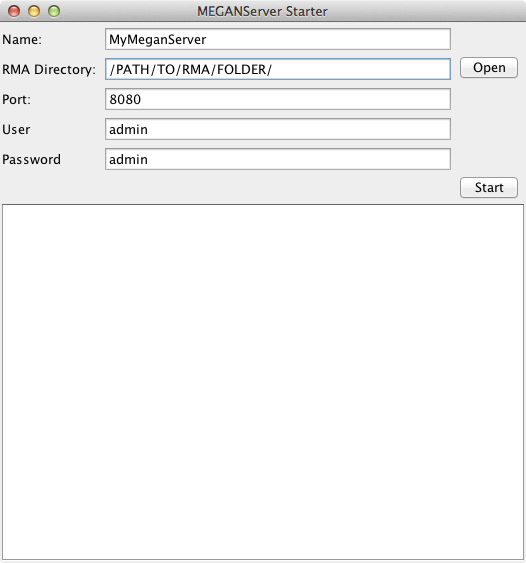
\includegraphics[width=0.49\textwidth]{ServerStarter1.png}
    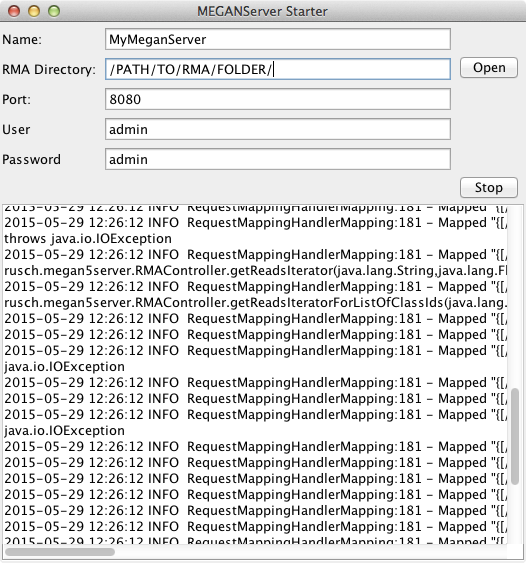
\includegraphics[width=0.49\textwidth]{ServerStarter2.png}
    \caption{Graphical user interface to start MEGANServer. MEGANServer accessible under \url{http://localhost:8080/MyMeganServer/}}
    \label{fig:starter}
\end{figure}


\subsection{Web Archive}
\textbf{Prerequisites}: MEGANServer requires an installed JAVA runtime (at least version 7). Furthermore a servlet container such as Tomcat or Jetty must be installed.

Download \texttt{MEGANServer\_webarchive.zip} from \url{http://ab.inf.uni-tuebingen.de/data/software/meganserver/download/MEGANServer\_webarchive.zip}. The archive includes:

\begin{itemize}
\item \texttt{MEGANServer.war}: The web archive containing the application and configuration files
\item \textbf{manual.pdf}: This manual
\end{itemize}


The application has to be launched inside a servlet engine such as Tomcat (see \url{http://tomcat.apache.org/}) or Jetty (see: \url{http://www.eclipse.org/jetty/}). Configuration as described in Section \ref{sec:config} takes place after the first launch. Optionally unzip the war file and edit the config files in the \textit{WEB-INF/classes/} folder before the first launch.

\section{Configuration}
\label{sec:config}

\subsection{Find metagenomic datasets}
\label{subsec:props}

MEGAN operates on so called Read Match Archives (short RMA), a binary file format that incorporates reads, matches, metadata and classification data and is currently available in version 2 and 3. This file structure is also being used by MEGANServer in order to publish data via the web service. That is why MEGANServer must be started with a base directory which will then be recursively searched for RMA2 and RMA3 files.
The base folder can be changed by modifying the entry \texttt{rma.rootFolder} in the \textit{MEGANServer.properties} file. MEGANServer will then find RMA files in this folder and all subfolders and expose those via the web service. This property can be set before starting the server or while running. For the latter option one must then reload the properties file by calling the method described in \ref{subsubsec:upProp}.


\subsection{Where to store the log files}
\textbf{Applicable only when using the webarchive version}

MEGANServer creates by default a log file in the folder where the web application is launched. The location of this file can be changed by altering the property \texttt{log4j.appender.file.File} in the \textit{log4.properties} file. This operation requires a restart of the web application.

\subsection{Altering user credentials}

The \textit{credentials.txt} file contains information about all users that are allowed to access a MEGANServer instance. Its entries can be changed either by editing the file (md5 hashed) or via web service using the commands as described in Section \ref{subsubsec:userInterface}.

The default user with administrative permissions has the username/password \textit{admin}. It is advisable to change the password of this user before the first start of the server.




\subsection{Information Text}

The \textit{info.txt} gives administrators the possibility to share information, such as what data is stored on the server and/or who to send an email for account requests. The \textit{info.txt} can be found together with the other configuration files and can contain either plaintext or html.

\section{MEGAN}

The metagenomics analysis tool MEGAN (\url{http://ab.inf.uni-tuebingen.de/software/megan5/}) comes with a graphical user interface to connect and exchange data with MEGANServer. With this connection one can work on remote datasets just as if they would be present on a local hard drive. Please read the MEGANServer section in the MEGAN manual for further information.


\section{MEGANServer REST API}
\subsection{Parameter}

The API uses queries to retrieve data. The selection of data is performed by methods and parameters. Since some parameters are recurring in multiple methods we will introduce in this section the parameters and in the next section the methods.


\subsubsection{Identifier}

MEGANServer accesses datasets and data inside datasets with unique identifier. There are three types of identifier.

\paragraph{Dataset/File Identifier}
\label{subsec:fileid}

The dataset/file identifier uniquely identifies a single dataset on a MEGANServer instance. The parameter on the API is \texttt{fileId} and is either a number such as \textbf{217396908} or the path to the dataset on the server such as \textbf{core1\_activelayer\_day2.rma}

\paragraph{Read Identifier}
\label{subsec:readuid}

Each read inside a dataset has a numerical identifier. This identifier is unique inside a dataset but the identifier is not required to be unique among datasets. Two different datasets can have same read identifier. On the API we refer to the read identifier as \texttt{readUid}.

\paragraph{Match Identifier}
\label{subsec:matchuid}

Each match inside a read has a numerical identifier. This identifier is unique inside a dataset but the identifier is not required to be unique among datasets. Two different datasets can have the same read identifier. On the API we refer to the match identifier as \texttt{matchUid}.


\subsubsection{General Parameters}

\paragraph{DataSelection}
\label{subsec:datasel}

When requesting reads or matches one can select which data fields should be returned. Currently following values are supported:


\texttt{useRead, useReadName, useReadHeader, useReadSequence, useMateUId, useReadLength, useReadComplexity, useReadNumberOfMatches, useMatchText, useMatchIgnore, useMatchBitScore, useMatchLength, useMatchTaxonId, useMatchSeedId, useMatchKeggId, useMatchCogId, useMatchExpected, useMatchRefSeq}

Therefore the parameter \texttt{dataSelection="useReadName,useReadLength"} would tell MEGANServer to return only the read name and the read length for a given query. If this parameter is skipped MEGANServer will use the default value which returns all possible data fields.






\paragraph{FindSelection and regEx}
\label{subsec:findsel}
MEGANServer supports searching for data matching regular expressions inside datasets. One has to specify where to search (FindSelection) and what to search for (regEx).

The FindSelection currently supports four data fields that can be searched:

\texttt{useMatchText, useReadHeader, useReadName, useReadSequence}

The regular expression can be any string or normal regular expression (See MEGAN manual for further information). 

A possible combination of these both parameters which returns data on all sequences that look like "ACTG" would then be \texttt{FindSelection="userReadSequence"\&regEx="ACTG"}




\paragraph{minScore and maxExpected}
\label{subsec:minScore}
These both parameters are meant to give users the possibility to filter matches by quality. The minScore parameter defines the minimal bitscore an alignment must have in order to appear in the results. The maxExpected value allows users to filter by E-Value. A possible parameter combination would be \texttt{minScore="100"\&maxExpected="0.0001"}.

The default values are for minScore 0 and for maxExpected 100000.


\paragraph{classification and classId(s)}
\label{subsec:class}
These both parameters are meant to give users the possibility to filter matches by classification and classification ids. MEGAN currently supports four classifications, namely NCBI taxonomy, SEED, COG and KEGG. Each of these classifications has identifier for e.g genes or taxa. Therefore the parameter \texttt{classification="Taxonomy"\&classId="562"} will tell the executing method to only return reads that stem from E.coli.



\subsection{General}
\subsubsection{help}

\begin{itemize}
	\item \textbf{Name}: help
	\item \textbf{Outline}: Get a list of all accessible commands of MEGANServer
	\item \textbf{Parameters}
		\begin{itemize}
			\item No Parameters
		\end{itemize}
	\item \textbf{Examples}:
		\begin{itemize}	
			\item \url{http://megan-db.org/Permafrost/}
			\item \url{http://megan-db.org/Permafrost/help}
		\end{itemize}
\end{itemize}

\subsubsection{info}

\begin{itemize}
	\item \textbf{Name}: info
	\item \textbf{Outline}: Get information about the data stored on this MEGANServer instance
	\item \textbf{Parameters}
		\begin{itemize}
			\item No Parameters
		\end{itemize}
	\item \textbf{Examples}:
		\begin{itemize}	
			\item \url{http://megan-db.org/Permafrost/info}
		\end{itemize}
\end{itemize}

\subsubsection{about}

\begin{itemize}
	\item \textbf{Name}: about
	\item \textbf{Outline}: Get a version number, contact information and build date of MEGANServer
	\item \textbf{Parameters}
		\begin{itemize}
			\item No Parameters
		\end{itemize}
	\item \textbf{Examples}:
		\begin{itemize}	
			\item \url{http://megan-db.org/Permafrost/About}
		\end{itemize}
\end{itemize}

\subsection{Reading RMA files}

\subsubsection{listDatasets}
\begin{itemize}
	\item \textbf{Name}: listDatasets
	\item \textbf{Outline}: Retrieve a list of datasets that is known to the MEGANServer instance.
	\item \textbf{Parameters}
		\begin{itemize}
			\item \textbf{includeMetadata}		
				\begin{itemize}
					\item \textbf{Name}: includeMetadata
					\item \textbf{Outline}: include metadata to the result
					\item \textbf{Required} : false
					\item \textbf{Default Value} : false
				\end{itemize}
		\end{itemize}
	\item \textbf{Examples}:
		\begin{itemize}
			\item \url{http://megan-db.org/Permafrost/listDatasets}			
			\item \url{http://megan-db.org/Permafrost/listDatasets?includeMetadata=True}
		\end{itemize}
\end{itemize}

\subsubsection{getFileUid}

\begin{itemize}
	\item \textbf{Name}: getFileUid
	\item \textbf{Outline}: Get the unique identifier for a dataset
	\item \textbf{Parameters}
		\begin{itemize}
			\item \textbf{fileId}		
				\begin{itemize}
					\item \textbf{Name}: fileId (see \ref{subsec:fileid})
					\item \textbf{Outline}: An identifier of a dataset. Either a path, a name or a number
					\item \textbf{Required} : true
					\item \textbf{Default Value} : --
				\end{itemize}
		\end{itemize}
	\item \textbf{Examples}:
		\begin{itemize}		
			\item \url{http://megan-db.org/Permafrost/getFileUid?fileId=core1_activelayer_day2.rma}
			\item \url{http://megan-db.org/Permafrost/getFileUid?fileId=217396908}			
		\end{itemize}
\end{itemize}

\subsubsection{getAuxiliary}

\begin{itemize}
	\item \textbf{Name}: getAuxiliary
	\item \textbf{Outline}: Get metadata and taxonomic/functional overview on a single dataset
	\item \textbf{Parameters}
		\begin{itemize}
			\item \textbf{fileId}
				\begin{itemize}
					\item \textbf{Name}: fileId (see \ref{subsec:fileid})
					\item \textbf{Outline}: An identifier of a dataset. Either a path, a name or a number
					\item \textbf{Required} : true
					\item \textbf{Default Value} : --
				\end{itemize}
		\end{itemize}
	\item \textbf{Examples}:
		\begin{itemize}		
			\item \url{http://megan-db.org/Permafrost/getAuxiliary?fileId=core1_activelayer_day2.rma}
		\end{itemize}
\end{itemize}

\subsubsection{getRead}

\begin{itemize}
	\item \textbf{Name}: getRead
	\item \textbf{Outline}: Get data on a single sequence together with all its information
	\item \textbf{Parameters}
		\begin{itemize}
			\item \textbf{fileId}		
				\begin{itemize}
					\item \textbf{Name}: fileId (see \ref{subsec:fileid})
					\item \textbf{Outline}: An identifier of a dataset. Either a path, a name or a number
					\item \textbf{Required} : true
					\item \textbf{Default Value} : --
				\end{itemize}
			\item \textbf{readUid}		
				\begin{itemize}
					\item \textbf{Name}: readUid (see \ref{subsec:readuid}) 
					\item \textbf{Outline}: The numerical identifier of the read
					\item \textbf{Required} : true
					\item \textbf{Default Value} : 0
				\end{itemize}
			\item \textbf{minScore}		
				\begin{itemize}
					\item \textbf{Name}: minScore (see \ref{subsec:minScore})
					\item \textbf{Outline}: The minimal bitscore a match has to have in order to be present in the result
					\item \textbf{Required} : false
					\item \textbf{Default Value} : 0
				\end{itemize}
			\item \textbf{maxExpected}		
				\begin{itemize}
					\item \textbf{Name}: maxExpected (see \ref{subsec:minScore})
					\item \textbf{Outline}: The maximal E-Value a match is allowed to have in order to be present in the result
					\item \textbf{Required} : false
					\item \textbf{Default Value} : 100000
				\end{itemize}
			\item \textbf{dataSelection}		
				\begin{itemize}
					\item \textbf{Name}: dataSelection (see \ref{subsec:datasel})
					\item \textbf{Outline}: Definition of fields that should be present in the result
					\item \textbf{Required} : false
					\item \textbf{Default Value} : useRead,useReadName,useReadHeader,useReadSequence, useMateUId,useReadLength,useReadComplexity,useReadNumberOfMatches, useMatchText,useMatchIgnore,useMatchBitScore,useMatchLength, useMatchTaxonId,useMatchSeedId,useMatchKeggId,useMatchCogId,useMatchExpected, useMatchRefSeq
				\end{itemize}
		\end{itemize}
	\item \textbf{Examples}:
		\begin{itemize}		
			\item \url{http://megan-db.org/Permafrost/getRead?fileId=217396908&readUid=331}
			\item \url{http://megan-db.org/Permafrost/getRead?fileId=217396908&readUid=643&minScore=10}
			\item \url{http://megan-db.org/Permafrost/getRead?fileId=217396908&readUid=643&minScore=10&maxExpected=0.01&dataSelection="useReadName,useReadLength"}
		\end{itemize}
\end{itemize}








\subsubsection{getAllReadsIterator}
\begin{itemize}
	\item \textbf{Name}: getAllReadIterator
	\item \textbf{Outline}: Get data of all reads of a single dataset. Returns one page of results and a link to the next page of results.
	\item \textbf{Parameters}
		\begin{itemize}
			\item \textbf{fileId}		
				\begin{itemize}
					\item \textbf{Name}: fileId (see \ref{subsec:fileid})
					\item \textbf{Outline}: An identifier of a dataset. Either a path, a name or a number
					\item \textbf{Required} : true
					\item \textbf{Default Value} : --
				\end{itemize}
			\item \textbf{minScore}		
				\begin{itemize}
					\item \textbf{Name}: minScore (see \ref{subsec:minScore})
					\item \textbf{Outline}: The minimal bitscore a match has to have in order to be present in the result
					\item \textbf{Required} : false
					\item \textbf{Default Value} : 0
				\end{itemize}
			\item \textbf{maxExpected}		
				\begin{itemize}
					\item \textbf{Name}: maxExpected (see \ref{subsec:minScore})
					\item \textbf{Outline}: The maximal E-Value a match is allowed to have in order to be present in the result
					\item \textbf{Required} : false
					\item \textbf{Default Value} : 100000
				\end{itemize}
			\item \textbf{dataSelection}		
				\begin{itemize}
					\item \textbf{Name}: dataSelection (see \ref{subsec:datasel})
					\item \textbf{Outline}: Definition of fields that should be present in the result
					\item \textbf{Required} : false
					\item \textbf{Default Value} : useRead,useReadName,useReadHeader,useReadSequence, useMateUId,useReadLength,useReadComplexity,useReadNumberOfMatches, useMatchText,useMatchIgnore,useMatchBitScore,useMatchLength, useMatchTaxonId,useMatchSeedId,useMatchKeggId,useMatchCogId,useMatchExpected, useMatchRefSeq
				\end{itemize}
		\end{itemize}
	\item \textbf{Examples}:
		\begin{itemize}		
			\item \url{http://megan-db.org/Permafrost/getAllReadsIterator?fileId=core1_activelayer_day2.rma}
		\end{itemize}
\end{itemize}

\subsubsection{getReadsIterator}
\begin{itemize}
	\item \textbf{Name}: getReadIterator
	\item \textbf{Outline}: Get data of all reads of a single dataset that are assigned to a node in the taxonomy or functional classification. Returns one page of results and a link to the next page of results.
	\item \textbf{Parameters}
		\begin{itemize}
			\item \textbf{fileId}		
				\begin{itemize}
					\item \textbf{Name}: fileId (see \ref{subsec:fileid})
					\item \textbf{Outline}: An identifier of a dataset. Either a path, a name or a number
					\item \textbf{Required} : true
					\item \textbf{Default Value} : --
				\end{itemize}
			\item \textbf{classId}		
				\begin{itemize}
					\item \textbf{Name}: classId (see \ref{subsec:class})
					\item \textbf{Outline}: The id of a classification such as NCBI taxonomy, KEGG or SEED
					\item \textbf{Required} : true
					\item \textbf{Default Value} : --
				\end{itemize}
			\item \textbf{classification}		
				\begin{itemize}
					\item \textbf{Name}: classification (see \ref{subsec:class})
					\item \textbf{Outline}: One of the classifications MEGAN supports
					\item \textbf{Required} : true
					\item \textbf{Default Value} : --
				\end{itemize}
			\item \textbf{minScore}		
				\begin{itemize}
					\item \textbf{Name}: minScore (see \ref{subsec:minScore})
					\item \textbf{Outline}: The minimal bitscore a match has to have in order to be present in the result
					\item \textbf{Required} : false
					\item \textbf{Default Value} : 0
				\end{itemize}
			\item \textbf{maxExpected}		
				\begin{itemize}
					\item \textbf{Name}: maxExpected (see \ref{subsec:minScore})
					\item \textbf{Outline}: The maximal E-Value a match is allowed to have in order to be present in the result
					\item \textbf{Required} : false
					\item \textbf{Default Value} : 100000
				\end{itemize}
			\item \textbf{dataSelection}		
				\begin{itemize}
					\item \textbf{Name}: dataSelection (see \ref{subsec:datasel})
					\item \textbf{Outline}: Definition of fields that should be present in the result
					\item \textbf{Required} : false
					\item \textbf{Default Value} : useRead,useReadName,useReadHeader,useReadSequence, useMateUId,useReadLength,useReadComplexity,useReadNumberOfMatches, useMatchText,useMatchIgnore,useMatchBitScore,useMatchLength, useMatchTaxonId,useMatchSeedId,useMatchKeggId,useMatchCogId,useMatchExpected, useMatchRefSeq
				\end{itemize}
		\end{itemize}
	\item \textbf{Examples}:
		\begin{itemize}		
			\item \url{http://megan-db.org/Permafrost/getReadsIterator?fileId=core1_activelayer_day2.rma&classification=Taxonomy&classId=14}
		\end{itemize}
\end{itemize}


\subsubsection{getReadsForMultipleClassIds}

\begin{itemize}
	\item \textbf{Name}: getReadsForMultipleClassIds
	\item \textbf{Outline}: Get data of all reads of a single dataset that are assigned to a number of nodes in the taxonomy or functional classification. Returns one page of results and a link to the next page of results.
	\item \textbf{Parameters}
		\begin{itemize}
			\item \textbf{fileId}		
				\begin{itemize}
					\item \textbf{Name}: fileId (see \ref{subsec:fileid})
					\item \textbf{Outline}: An identifier of a dataset. Either a path, a name or a number
					\item \textbf{Required} : true
					\item \textbf{Default Value} : --
				\end{itemize}
			\item \textbf{classId}		
				\begin{itemize}
					\item \textbf{Name}: classId (see \ref{subsec:class})s
					\item \textbf{Outline}: The ids of a classification such as NCBI taxonomy, KEGG or SEED
					\item \textbf{Required} : true
					\item \textbf{Default Value} : --
				\end{itemize}
			\item \textbf{classification}		
				\begin{itemize}
					\item \textbf{Name}: classification (see \ref{subsec:class})
					\item \textbf{Outline}: One of the classifications MEGAN supports
					\item \textbf{Required} : true
					\item \textbf{Default Value} : --
				\end{itemize}
			\item \textbf{minScore}		
				\begin{itemize}
					\item \textbf{Name}: minScore (see \ref{subsec:minScore})
					\item \textbf{Outline}: The minimal bitscore a match has to have in order to be present in the result
					\item \textbf{Required} : false
					\item \textbf{Default Value} : 0
				\end{itemize}
			\item \textbf{maxExpected}		
				\begin{itemize}
					\item \textbf{Name}: maxExpected (see \ref{subsec:minScore})
					\item \textbf{Outline}: The maximal E-Value a match is allowed to have in order to be present in the result
					\item \textbf{Required} : false
					\item \textbf{Default Value} : 100000
				\end{itemize}
			\item \textbf{dataSelection}		
				\begin{itemize}
					\item \textbf{Name}: dataSelection (see \ref{subsec:datasel})
					\item \textbf{Outline}: Definition of fields that should be present in the result
					\item \textbf{Required} : false
					\item \textbf{Default Value} : useRead,useReadName,useReadHeader,useReadSequence, useMateUId,useReadLength,useReadComplexity,useReadNumberOfMatches, useMatchText,useMatchIgnore,useMatchBitScore,useMatchLength, useMatchTaxonId,useMatchSeedId,useMatchKeggId,useMatchCogId,useMatchExpected, useMatchRefSeq
				\end{itemize}
		\end{itemize}
	\item \textbf{Examples}:
		\begin{itemize}		
			\item \url{http://megan-db.org/Permafrost/getReadsForMultipleClassIds?fileId=core1_activelayer_day2.rma&classification=Taxonomy&classIds=14,-1}
		\end{itemize}
\end{itemize}
\subsubsection{getFindAllReadsIterator}


\begin{itemize}
	\item \textbf{Name}: getFindAllReadIterator
	\item \textbf{Outline}: Get data of all reads of a single dataset and searches for text patterns. Those fulfilling the pattern are returned. Returns one page of results and a link to the next page of results.
	\item \textbf{Parameters}
		\begin{itemize}
			\item \textbf{fileId}		
				\begin{itemize}
					\item \textbf{Name}: fileId (see \ref{subsec:fileid})
					\item \textbf{Outline}: An identifier of a dataset. Either a path, a name or a number
					\item \textbf{Required} : true
					\item \textbf{Default Value} : --
				\end{itemize}
			\item \textbf{regEx}		
				\begin{itemize}
					\item \textbf{Name}: regEx (see \ref{subsec:findsel})
					\item \textbf{Outline}: Regular expression that is being searched for
					\item \textbf{Required} : true
					\item \textbf{Default Value} : --
				\end{itemize}
			\item \textbf{findSelection}		
				\begin{itemize}
					\item \textbf{Name}: findSelection (see \ref{subsec:findsel})
					\item \textbf{Outline}: Where to search
					\item \textbf{Required} : false
					\item \textbf{Default Value} : useMatchText,useReadHeader,useReadName,useReadSequence
				\end{itemize}

		\end{itemize}
	\item \textbf{Examples}:
		\begin{itemize}		
			\item \url{http://megan-db.org/Permafrost/getFindAllReadsIterator?fileId=core1_activelayer_day2.rma&regEx=Bacteria&findSelection=useMatchText}
		\end{itemize}
\end{itemize}


\subsubsection{loadPagedReads}

\begin{itemize}
	\item \textbf{Name}: loadPagedReads
	\item \textbf{Outline}: Load the next page of an readblockiterator
	\item \textbf{Parameters}
		\begin{itemize}
			\item \textbf{pageId}		
				\begin{itemize}
					\item \textbf{Name}: pageId
					\item \textbf{Outline}: Next page Id. Retrieved from the previous page
					\item \textbf{Required} : true
					\item \textbf{Default Value} : --
				\end{itemize}
		\end{itemize}
	\item \textbf{Examples}: \textcolor{red}{Pages and pageIds are dynamic. This is why the link in the example will not work. Try to insert your own pageId.}
		\begin{itemize}		
			\item \url{http://megan-db.org/Permafrost/loadPagedReads?pageId=823880593}
		\end{itemize}
\end{itemize}


\subsubsection{getNumberOfReads}

\begin{itemize}
	\item \textbf{Name}: getNumberOfReads
	\item \textbf{Outline}: Get number of reads for one dataset
	\item \textbf{Parameters}
		\begin{itemize}
			\item \textbf{fileId}		
				\begin{itemize}
					\item \textbf{Name}: fileId (see \ref{subsec:fileid})
					\item \textbf{Outline}: An identifier of a dataset. Either a path, a name or a number
					\item \textbf{Required} : true
					\item \textbf{Default Value} : --
				\end{itemize}
		\end{itemize}
	\item \textbf{Examples}:
		\begin{itemize}		
			\item \url{http://megan-db.org/Permafrost/getNumberOfReads?fileId=217396908}
		\end{itemize}
\end{itemize}


\subsubsection{getNumberOfMatches}

\begin{itemize}
	\item \textbf{Name}: getNumberOfMatches
	\item \textbf{Outline}: Get number of alignments for one dataset
	\item \textbf{Parameters}
		\begin{itemize}
			\item \textbf{fileId}		
				\begin{itemize}
					\item \textbf{Name}: fileId (see \ref{subsec:fileid})
					\item \textbf{Outline}: An identifier of a dataset. Either a path, a name or a number
					\item \textbf{Required} : true
					\item \textbf{Default Value} : --
				\end{itemize}
		\end{itemize}
	\item \textbf{Examples}:
		\begin{itemize}		
			\item \url{http://megan-db.org/Permafrost/getNumberOfMatches?fileId=217396908}
		\end{itemize}
\end{itemize}


\subsubsection{getAllClassificationNames}
\begin{itemize}
	\item \textbf{Name}: getAllClassifcationNames
	\item \textbf{Outline}: Get the names of all classifications present in this dataset
	\item \textbf{Parameters}
		\begin{itemize}
			\item \textbf{fileId}		
				\begin{itemize}
					\item \textbf{Name}: fileId (see \ref{subsec:fileid})
					\item \textbf{Outline}: An identifier of a dataset. Either a path, a name or a number
					\item \textbf{Required} : true
					\item \textbf{Default Value} : --
				\end{itemize}
		\end{itemize}
	\item \textbf{Examples}:
		\begin{itemize}		
			\item \url{http://megan-db.org/Permafrost/getAllClassificationNames?fileId=core1_activelayer_day2.rma}
		\end{itemize}
\end{itemize}
\subsubsection{getClassSize}
\begin{itemize}
	\item \textbf{Name}: getClassSize
	\item \textbf{Outline}: Get the number of reads assigned to one node in a classification
	\item \textbf{Parameters}
		\begin{itemize}
			\item \textbf{fileId}		
				\begin{itemize}
					\item \textbf{Name}: fileId (see \ref{subsec:fileid})
					\item \textbf{Outline}: An identifier of a dataset. Either a path, a name or a number
					\item \textbf{Required} : true
					\item \textbf{Default Value} : --
				\end{itemize}
			\item \textbf{classId}		
				\begin{itemize}
					\item \textbf{Name}: classId (see \ref{subsec:class})
					\item \textbf{Outline}: The id of a classification such as NCBI taxonomy, KEGG or SEED
					\item \textbf{Required} : true
					\item \textbf{Default Value} : --
				\end{itemize}
			\item \textbf{classification}		
				\begin{itemize}
					\item \textbf{Name}: classification (see \ref{subsec:class})
					\item \textbf{Outline}: One of the classifications MEGAN supports
					\item \textbf{Required} : true
					\item \textbf{Default Value} : --
				\end{itemize}
		\end{itemize}
	\item \textbf{Examples}:
		\begin{itemize}		
			\item \url{http://megan-db.org/Permafrost/getClassSize?fileId=core1_activelayer_day2.rma&classification=Taxonomy&classId=14}
		\end{itemize}
\end{itemize}

\subsubsection{getClassificationBlock}

\begin{itemize}
	\item \textbf{Name}: getClassificationBlock
	\item \textbf{Outline}: Get the number of reads assigned to all nodes in a classification
	\item \textbf{Parameters}
		\begin{itemize}
			\item \textbf{fileId}		
				\begin{itemize}
					\item \textbf{Name}: fileId (see \ref{subsec:fileid})
					\item \textbf{Outline}: An identifier of a dataset. Either a path, a name or a number
					\item \textbf{Required} : true
					\item \textbf{Default Value} : --
				\end{itemize}
			\item \textbf{classification}		
				\begin{itemize}
					\item \textbf{Name}: classification (see \ref{subsec:class})
					\item \textbf{Outline}: One of the classifications MEGAN supports
					\item \textbf{Required} : true
					\item \textbf{Default Value} : --
				\end{itemize}
		\end{itemize}
	\item \textbf{Examples}:
		\begin{itemize}		
			\item \url{http://megan-db.org/Permafrost/getClassificationBlock?fileId=core1_activelayer_day2.rma&classification=Taxonomy}
		\end{itemize}
\end{itemize}

\subsubsection{isReadOnly}

\begin{itemize}
	\item \textbf{Name}: isReadOnly
	\item \textbf{Outline}: Determines if user has write permissions. Currently all datasets are readOnly, no matter if a user is admin or not.
	\item \textbf{Parameters}
		\begin{itemize}
			\item \textbf{fileId}		
				\begin{itemize}
					\item \textbf{Name}: fileId (see \ref{subsec:fileid})
					\item \textbf{Outline}: An identifier of a dataset. Either a path, a name or a number
					\item \textbf{Required} : true
					\item \textbf{Default Value} : --
				\end{itemize}
		\end{itemize}
	\item \textbf{Examples}:
		\begin{itemize}		
			\item \url{http://megan-db.org/Permafrost/isReadOnly?fileId=core1_activelayer_day2.rma}
		\end{itemize}
\end{itemize}

\subsubsection{getClassificationSize}
\begin{itemize}
	\item \textbf{Name}: getClassificationSize
	\item \textbf{Outline}: Get the number of nodes with reads in a classification
	\item \textbf{Parameters}
		\begin{itemize}
			\item \textbf{fileId}		
				\begin{itemize}
					\item \textbf{Name}: fileId (see \ref{subsec:fileid})
					\item \textbf{Outline}: An identifier of a dataset. Either a path, a name or a number
					\item \textbf{Required} : true
					\item \textbf{Default Value} : --
				\end{itemize}
			\item \textbf{classification}		
				\begin{itemize}
					\item \textbf{Name}: classification (see \ref{subsec:class})
					\item \textbf{Outline}: One of the classifications MEGAN supports
					\item \textbf{Required} : true
					\item \textbf{Default Value} : --
				\end{itemize}
		\end{itemize}
	\item \textbf{Examples}:
		\begin{itemize}		
			\item \url{http://megan-db.org/Permafrost/getClassificationSize?fileId=core1_activelayer_day2.rma&classification=Taxonomy}
		\end{itemize}
\end{itemize}

\subsection{Admin}
\textcolor{red}{Accessible with admin permission only!}
\subsubsection{admin/updateDatasets}
\label{subsubsec:upProp}
\begin{itemize}
	\item \textbf{Name}: admin/updateDatasets
	\item \textbf{Outline}: Reads the root location from the \textit{MEGANServer.properties} file and updates the list of datasets
	\item \textbf{Parameters}
		\begin{itemize}
			\item  None
		\end{itemize}
	\item \textbf{Examples}:
		\begin{itemize}		
			\item \url{http://megan-db.org/Permafrost/admin/updateDatasets}
		\end{itemize}
\end{itemize}



\subsubsection{admin/addUser}

\begin{itemize}
	\item \textbf{Name}: addUser
	\item \textbf{Outline}: Get the number of nodes with reads in a classification
	\item \textbf{Parameters}
		\begin{itemize}
			\item \textbf{userName}		
				\begin{itemize}
					\item \textbf{Name}: userName
					\item \textbf{Outline}: Name of the new user
					\item \textbf{Required} : true
					\item \textbf{Default Value} : --
				\end{itemize}
			\item \textbf{password}		
				\begin{itemize}
					\item \textbf{Name}: password
					\item \textbf{Outline}: password for the user
					\item \textbf{Required} : true
					\item \textbf{Default Value} : --
				\end{itemize}
			\item \textbf{isAdmin}		
				\begin{itemize}
					\item \textbf{Name}: isAdmin
					\item \textbf{Outline}: Determines if the new user should get admin rights
					\item \textbf{Required} : true
					\item \textbf{Default Value} : --
				\end{itemize}
		\end{itemize}
	\item \textbf{Examples}:
		\begin{itemize}		
			\item \url{http://megan-db.org/Permafrost/admin/addUser?userName=Megan&password=Server&isAdmin=false}
		\end{itemize}
\end{itemize}

\subsubsection{admin/listUsers}
\label{subsubsec:userInterface}
\begin{itemize}
	\item \textbf{Name}: listUsers
	\item \textbf{Outline}: Get the list of active users
	\item \textbf{Parameters}
		\begin{itemize}
			\item No parameters
		\end{itemize}
	\item \textbf{Examples}:
		\begin{itemize}		
			\item \url{http://megan-db.org/Permafrost/admin/listUsers}
		\end{itemize}
\end{itemize}
\subsubsection{admin/removeUser}
\begin{itemize}
	\item \textbf{Name}: admin/removeUser
	\item \textbf{Outline}: Delete user and revoke credentials
	\item \textbf{Parameters}
		\begin{itemize}
			\item \textbf{userName}		
				\begin{itemize}
					\item \textbf{Name}: userName
					\item \textbf{Outline}: Name of the new user
					\item \textbf{Required} : true
					\item \textbf{Default Value} : --
				\end{itemize}
		\end{itemize}
	\item \textbf{Examples}:
		\begin{itemize}		
			\item \url{http://megan-db.org/Permafrost/admin/removeUser?userName=Megan}
		\end{itemize}
\end{itemize}
\subsubsection{admin/getLog}

\begin{itemize}
	\item \textbf{Name}: admin/getLog
	\item \textbf{Outline}: Returns log entries
	\item \textbf{Parameters}
		\begin{itemize}
			\item No parameters
		\end{itemize}
	\item \textbf{Examples}:
		\begin{itemize}		
			\item \url{http://megan-db.org/Permafrost/admin/getLog}
		\end{itemize}
\end{itemize}

\section{Acknowledgements}

This research is supported by the German Federal Ministry of Education and Research.

\bibliographystyle{natbib}
\begin{thebibliography}{}


\bibitem[Huson {\em et~al.}(2011)Huson, Mitra, Weber, Ruscheweyh, and
  Schuster]{MEGAN2011}
Huson, D.~H., Mitra, S., Weber, N., Ruscheweyh, H.-J., and Schuster, S.~C.
  (2011).
\newblock Integrative analysis of environmental sequences using {MEGAN\,4}.
\newblock {\em Genome Research\/}, {\bf 21}, 1552--1560.

\bibitem[Mackelprang {\em et~al.}(2011)Mackelprang, Waldrop, DeAngelis, David,
  Chavarria, Blazewicz, Rubin, and Jansson]{Mackelprang2011}
Mackelprang, R., Waldrop, M., DeAngelis, K., David, M., Chavarria, K.,
  Blazewicz, S., Rubin, E., and Jansson, J. (2011).
\newblock Metagenomic analysis of a permafrost microbial community reveals a
  rapid response to thaw.
\newblock {\em Nature\/}, {\bf 480}(7377), 368--371.

\end{thebibliography}


\end{document}